\documentclass[11pt]{article}

\usepackage[margin=1in]{geometry}
\usepackage{amsmath,amssymb}
\usepackage{graphicx}
\usepackage{xcolor}
\usepackage[numbers,sort&compress]{natbib}
\usepackage{xurl}
\usepackage{enumitem}
\setlist{noitemsep,topsep=3pt}               % compact lists
\setlength{\bibsep}{2pt}                     % compact bibliography
\usepackage{titling}
\setlength{\droptitle}{-5em}                 % less empty space above the title
\usepackage[colorlinks=true,linkcolor=blue!60!black,citecolor=blue!60!black,urlcolor=blue!60!black]{hyperref}
\usepackage[capitalise,noabbrev]{cleveref}

\graphicspath{{figures/}}

% Marks a section that is not written yet.
\newcommand{\inprogress}[1]{\noindent\textcolor{gray}{\textit{In progress: #1}}\par}

\newcommand{\Smax}{S_{\max}}
\newcommand{\Vmax}{V_{\max}}
\newcommand{\Lop}{\mathcal{L}}

\title{ADI Finite-Difference Methods for American Options\\under the Heston Model\\[6pt]
  \large Check-in report --- Math/CS 714, Fall 2026}
\author{Ganesh Arivoli \and Rohan Gupta\\[4pt]}
\date{November 16, 2026}

\begin{document}
\maketitle

% ===========================================================================
\section{Project goal}
% ===========================================================================
We explore alternating direction implicit (ADI) finite-difference methods for option pricing under the Heston
stochastic-volatility model \cite{heston1993}, and their implementation on parallel hardware. The Heston pricing
PDE is two-dimensional (stock price and variance) and has a mixed-derivative term. ADI methods split each time
step into cheap one-dimensional implicit steps, and the many independent tridiagonal solves in each step make
them a natural fit for multicore CPUs and GPUs. In this first phase we implemented four ADI schemes for European
puts and compared them with the semi-analytic Heston price. Next, we plan to implement the time-stepping loop on
the CPU (multithreaded C++) and on the GPU (CUDA) and compare their performance.

% ===========================================================================
\section{Background and prior work}
% ===========================================================================
\paragraph{The Heston model.}
Heston \cite{heston1993} models the variance $v$ of the stock as a mean-reverting square-root process whose
random shocks are correlated with those of the price. A negative correlation $\rho$ produces the skew seen in
equity option prices, which a constant-volatility model cannot reproduce. For European options the
characteristic function of the log-price is known in closed form, so prices reduce to one-dimensional
integrals. We compute our reference prices this way, using the formulation of Albrecher et
al.~\cite{albrecher2007}, which avoids jumps between branches of the complex logarithm, and we check it against
a published value of Fang and Oosterlee~\cite{fang2008}. American options have no closed-form price under the Heston
model, so they need a numerical method such as the finite-difference approach we take.

\paragraph{ADI schemes.}
ADI methods replace each implicit step of a multi-dimensional problem by implicit steps in one direction at a
time, each needing only tridiagonal solves (see \cite{inthout2010} and the references there for their
history). Each of these one-directional stages has a weight $\vartheta\in[0,1]$ that sets how implicit it is:
$\vartheta=0$ gives an explicit step, $\vartheta=1$ a fully implicit one, and $\vartheta=\tfrac12$ the
Crank--Nicolson average of the old and new values. A mixed-derivative term belongs to neither direction, so it has to be treated explicitly, and the
Douglas scheme then drops to first order in time. Craig and Sneyd~\cite{craig1988} added a correction stage
that restores second order. The Modified Craig--Sneyd and Hundsdorfer--Verwer schemes refine this correction
and remain second order for any $\vartheta$~\cite{inthout2010}. In 't Hout and
Foulon~\cite{inthout2010} applied all four schemes to the Heston PDE on non-uniform grids and found three of
them, Craig--Sneyd, Modified Craig--Sneyd and Hundsdorfer--Verwer, to be very effective. We follow their
formulation, and our default weights (\cref{tab:schemes}) come from this line of
work~\cite{inthout2010,haentjens2015}.

\paragraph{Non-smooth initial data.}
The payoff has a kink at $s=K$. Schemes of Crank--Nicolson type damp the high-frequency errors this creates only
weakly, and the errors show up as oscillations in the Greeks. Rannacher~\cite{rannacher1984} proposed starting
with a few fully implicit steps to damp them.

\paragraph{American options.}
The early-exercise constraint turns the pricing problem into the linear complementarity
problem~\eqref{eq:lcp} below. Ikonen and Toivanen~\cite{ikonen2009} split each time step into a linear step
followed by a cheap pointwise update of the solution and of a Lagrange multiplier, so the linear systems are
the same as for a European option. This fits the ADI framework, and Haentjens and in 't
Hout~\cite{haentjens2015} combined it with the four ADI schemes for American options under the Heston model.

\paragraph{Parallel computing.}
Every ADI stage solves many independent tridiagonal systems, one per grid line, which suits parallel hardware.
On a CPU the lines can be split across threads, and on a GPU each line can get its own thread running the
Thomas algorithm. Alternatively, one system can be split across many threads with cyclic reduction or parallel
cyclic reduction, as studied for GPUs by Zhang, Cohen and Owens~\cite{zhang2010}. Choosing between these is
part of the performance comparison we plan.

% ===========================================================================
\section{Problem}
% ===========================================================================
Let $u(s,v,\tau)$ be the option value as a function of the stock price $s$, the variance $v$ and the time to
maturity $\tau=T-t$. The payoff is known at maturity, so in $\tau$ it becomes an initial condition, and pricing
is a forward initial-value problem, like the heat equation with the payoff as the initial temperature.
For a European put with strike $K$, $u$ satisfies
\begin{equation}\label{eq:pde}
  u_\tau = \Lop u := \tfrac12 s^2 v\,u_{ss} + \rho\xi s v\,u_{sv} + \tfrac12\xi^2 v\,u_{vv}
  + (r-q)s\,u_s + \kappa(\theta-v)\,u_v - r u,
\end{equation}
with initial condition $u(s,v,0) = g(s) = \max(K-s,0)$. Here $r$ is the interest rate, $q$ the dividend yield, $\kappa$ the speed at which the variance returns to its
long-run level $\theta$, $\xi$ the volatility of the variance, and $\rho$ the correlation between price and
variance. \Cref{tab:terms} lists what each term describes. Setting $\xi=0$ and $v=\theta$ removes the
$v$-derivatives and gives back the Black--Scholes equation with volatility $\sqrt\theta$, which we use as a check.

\begin{table}[ht]
  \centering
  \caption{The terms of the Heston PDE~\eqref{eq:pde}.}
  \label{tab:terms}
  \begin{tabular}{ll}
    \hline
    Term & Meaning \\
    \hline
    $\tfrac12 s^2 v\,u_{ss}$ & diffusion in $s$: random price moves, with size set by $v$ \\
    $\rho\xi s v\,u_{sv}$ & mixed term: price and variance moves are correlated (zero if $\rho=0$) \\
    $\tfrac12\xi^2 v\,u_{vv}$ & diffusion in $v$: the variance itself is random \\
    $(r-q)s\,u_s$ & drift of the stock price \\
    $\kappa(\theta-v)\,u_v$ & the variance is pulled back toward $\theta$ \\
    $-ru$ & discounting \\
    \hline
  \end{tabular}
\end{table}

\paragraph{American options.}
An American put can be exercised at any time, so its value may not fall below the payoff $g$. At each point,
either holding is better and the PDE holds, or exercising is better and $u=g$. In one line,
\begin{equation}\label{eq:lcp}
  \min\bigl(u_\tau - \Lop u,\; u - g\bigr) = 0.
\end{equation}

\paragraph{Domain and boundary conditions.}
We solve on the truncated domain $[0,\Smax]\times[0,\Vmax]$ with $\Smax=8K$ and $\Vmax=5$.
These are the values chosen by in 't Hout and Foulon~\cite{inthout2010} for the Heston PDE.
\begin{itemize}
  \item $s=0$: the stock stays at $0$, so a European put pays $K$ at maturity, worth $u=Ke^{-r\tau}$ today.
  An American put is exercised at once, so there $u=K$.
  \item $s=\Smax$: far above the strike the put is nearly worthless and flat, so $u_s=0$.
  \item $v=\Vmax$: for very large variance the value barely changes with $v$, so $u_v=0$.
  \item $v=0$: all second-derivative terms vanish, and the PDE becomes
  $u_\tau=(r-q)s\,u_s+\kappa\theta\,u_v-ru$. Since $\kappa\theta>0$, values on this edge are determined by
  values at larger $v$, inside the domain: it is an outflow edge. So no boundary condition is needed, and we
  solve this reduced PDE on the edge itself.
\end{itemize}

% ===========================================================================
\section{Method and implementation}
% ===========================================================================
So far we have worked on European puts, which have a reference price to compare against.

\paragraph{Space discretization.}
We use non-uniform grids with more points near the strike $K$, where the payoff has a kink, and near $v=0$.
Derivatives are replaced by three-point central differences on the non-uniform grid, which are second-order
accurate when the grid spacing changes smoothly. Where a central difference for a first-derivative term would
give a negative off-diagonal coefficient (cell P\'eclet number above $2$), we switch to a first-order upwind
difference. This keeps the tridiagonal systems diagonally dominant, so the Thomas algorithm needs no pivoting.
On our test grids it happens only at large $v$ (from about $v=0.55$ on the $101\times51$ grid) and, in the
$s$-direction, at very small $v$, both away from where we read off the price. At $v=0$ we use a one-sided
difference for $u_v$. The mixed derivative $u_{sv}$ is approximated by combining
the first-derivative formulas in $s$ and $v$. We then split the discrete operator by direction,
\[
  A = A_0 + A_1 + A_2,
\]
where $A_0$ is the mixed term, $A_1$ contains the $s$-derivatives and $A_2$ the $v$-derivatives. $A_1$ and $A_2$
only couple neighbouring points along one grid line, so they are tridiagonal along that line.

\paragraph{Time discretization using ADI.}
After the space discretization we have a large system of ordinary differential equations,
\[
  U'(\tau) = A\,U(\tau) + b(\tau),
\]
where $U$ holds the values at all grid points and $b$ carries the boundary data. An explicit time-stepping
method is cheap per step but is only stable for $\Delta\tau$ of order $h^2$, which needs far too many steps.
A fully implicit method is stable for large steps but needs a large two-dimensional sparse solve at every step.
ADI methods sit in between: they are implicit in one direction at a time, so each step needs only tridiagonal
solves, one per grid line, which we do with the Thomas algorithm.

\paragraph{The Douglas scheme.}
One Douglas step from $U^{n-1}$ to $U^n$, with step size $\Delta\tau$ and weight $\vartheta$, is
(boundary data left out for readability):
\begin{align*}
  Y_0 &= U^{n-1} + \Delta\tau\,A\,U^{n-1} && \text{explicit predictor with all terms,}\\
  Y_1 &= Y_0 + \vartheta\Delta\tau\,A_1\,(Y_1 - U^{n-1}) && \text{implicit correction in } s,\\
  Y_2 &= Y_1 + \vartheta\Delta\tau\,A_2\,(Y_2 - U^{n-1}) && \text{implicit correction in } v,
\end{align*}
and $U^n=Y_2$. The second and third lines are the tridiagonal solves
$(I-\vartheta\Delta\tau A_j)\,Y_j = Y_{j-1} - \vartheta\Delta\tau A_j U^{n-1}$. We use $\vartheta$ for the ADI weight so that
it is not confused with the Heston parameter $\theta$.

\paragraph{The four ADI schemes.}
All four schemes start with the Douglas stages above. The other three then add a correction stage and repeat
the two implicit stages. With $Y_0$, $Y_1$, $Y_2$ from the Douglas step:
\begin{itemize}
  \item \textbf{Douglas.} $U^n=Y_2$. The mixed term $A_0$ enters only through the explicit predictor, a
  forward Euler step, so the scheme is first order in time when $\rho\neq0$, and second order when $\rho=0$
  and $\vartheta=\tfrac12$.
  \item \textbf{Craig--Sneyd.} Correct the mixed term with its average over the old and new values,
  $\tilde Y_0 = Y_0 + \tfrac12\Delta\tau\,A_0(Y_2-U^{n-1})$, then repeat the implicit stages from $\tilde Y_0$:
  $\tilde Y_j = \tilde Y_{j-1} + \vartheta\Delta\tau\,A_j(\tilde Y_j-U^{n-1})$ for $j=1,2$, and $U^n=\tilde Y_2$.
  This is second order for $\vartheta=\tfrac12$.
  \item \textbf{Modified Craig--Sneyd.} As Craig--Sneyd, but the correction also includes all of $A$:
  $\tilde Y_0 = Y_0 + \vartheta\Delta\tau\,A_0(Y_2-U^{n-1}) + (\tfrac12-\vartheta)\Delta\tau\,A(Y_2-U^{n-1})$.
  It is second order for every $\vartheta$, and reduces to Craig--Sneyd at $\vartheta=\tfrac12$.
  \item \textbf{Hundsdorfer--Verwer.} Correct all of $A$, $\tilde Y_0 = Y_0 + \tfrac12\Delta\tau\,A(Y_2-U^{n-1})$,
  then repeat the implicit stages relative to $Y_2$ instead of $U^{n-1}$:
  $\tilde Y_j = \tilde Y_{j-1} + \vartheta\Delta\tau\,A_j(\tilde Y_j-Y_2)$ for $j=1,2$, and $U^n=\tilde Y_2$.
  It is second order for every $\vartheta$.
\end{itemize}
Because Modified Craig--Sneyd and Hundsdorfer--Verwer are second order for every $\vartheta$, $\vartheta$ can be chosen for stability;
\cref{tab:schemes} lists the values we use. The second round of implicit stages makes the three corrected schemes about
twice as expensive per step as Douglas. We implemented all four schemes following \cite{inthout2010}.

\begin{table}[ht]
  \centering
  \caption{The four ADI schemes. The weights $\vartheta$ are the ones we use by default.}
  \label{tab:schemes}
  \begin{tabular}{lll}
    \hline
    Scheme & Correction after the Douglas step & $\vartheta$ \\
    \hline
    Douglas & none & $\tfrac12$ \\
    Craig--Sneyd & corrects $A_0$ using $Y_2$ & $\tfrac12$ \\
    Modified Craig--Sneyd & as Craig--Sneyd, plus a correction with all of $A$ & $\tfrac13$ \\
    Hundsdorfer--Verwer & corrects all of $A$ using $Y_2$ & $\tfrac12+\tfrac{\sqrt3}{6}$ \\
    \hline
  \end{tabular}
\end{table}

\paragraph{Start-up steps.}
The initial condition $g(s)=\max(K-s,0)$ is not smooth: its slope jumps from $-1$ to $0$ at $s=K$, and
on the grid this kink excites high-frequency error components. For very stiff modes the Crank--Nicolson
amplification factor approaches $-1$, so these errors flip sign every step instead of decaying, and they show up
as oscillations in $\Gamma=u_{ss}$. A fully implicit step has amplification factor approaching $0$ and damps
them.

\paragraph{Rannacher smoothing.}
Rannacher~\cite{rannacher1984} proposed taking the first few steps with the implicit Euler method, which damps
these modes, and then switching to the second-order method. Only a fixed number of steps use the first-order
method, so the overall order is not lowered. In our solver, the first full step of size $\Delta\tau$ is
replaced by two half-steps of size $\Delta\tau/2$ with the Douglas scheme at $\vartheta=1$, the ADI counterpart
of implicit Euler; all remaining steps use the chosen scheme with its weight from \cref{tab:schemes}.

\paragraph{Implementation.}
The solver is a Python package built on NumPy and SciPy. It has unit tests for every part, including checks
against the exact Black--Scholes price (the special case $\xi=0$) and against a semi-analytic Heston price
computed from the characteristic function \cite{heston1993}.

% ===========================================================================
\section{Preliminary results}
% ===========================================================================
We use the test case $r=0.025$, $q=0$, $\kappa=1.5$, $\theta=0.04$, $\xi=0.3$, $K=100$, $T=1$, with $\rho=0$ or
$\rho=-0.9$, and read off the price at $S_0=100$, $v_0=0.04$. \Cref{fig:convergence} shows the two main checks so far.

\begin{figure}[ht]
  \centering
  \begin{minipage}[t]{0.49\linewidth}
    \centering
    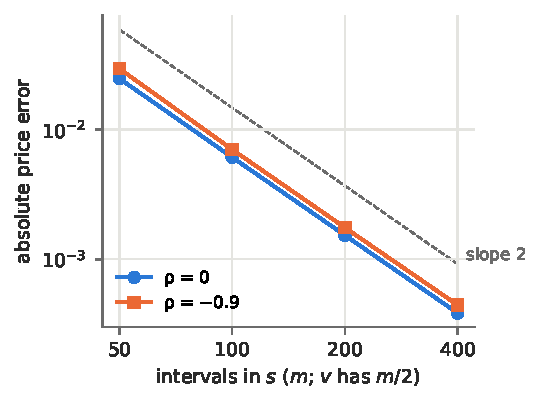
\includegraphics[width=0.9\linewidth]{space_convergence.pdf}\\
    \small (a) Error against the reference price.
  \end{minipage}\hfill
  \begin{minipage}[t]{0.49\linewidth}
    \centering
    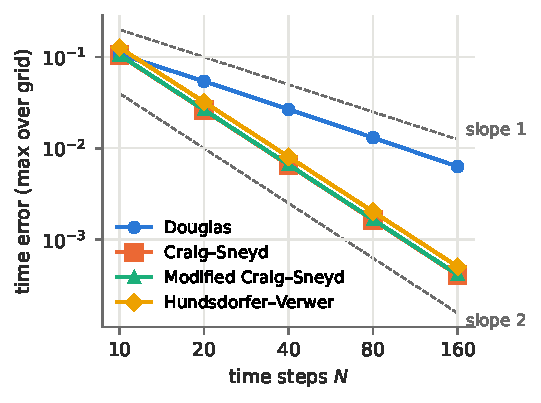
\includegraphics[width=0.9\linewidth]{time_convergence.pdf}\\
    \small (b) Time error, $\rho=-0.9$.
  \end{minipage}
  \caption{(a) Price error of the Craig--Sneyd scheme against the semi-analytic Heston price as the grid is
  refined, with $N=m$ time steps. (b) Time error of the four schemes on a fixed $61\times31$ grid, measured as the
  largest difference from a run with $2560$ steps. Craig--Sneyd and Modified Craig--Sneyd almost coincide.}
  \label{fig:convergence}
\end{figure}

\paragraph{Space.}
In \cref{fig:convergence}(a), the error falls by about a factor of $4$ each time the grid is refined, both
without correlation ($\rho=0$) and with strong correlation ($\rho=-0.9$). This is consistent with second-order
accuracy in space.

\paragraph{Time.}
In \cref{fig:convergence}(b), with $\rho=-0.9$, the Douglas error roughly halves when the number of steps
doubles, while the errors of the other three schemes fall by about a factor of $4$. This matches the expected
first-order behaviour of Douglas and second-order behaviour of the other schemes when the mixed term is present.

% ===========================================================================
\section{Remaining work}
% ===========================================================================
\begin{itemize}
  \item \textbf{Parallel implementation.} Port the time-stepping loop to multithreaded C++ and to CUDA.
  \item \textbf{American options.} Add the early-exercise constraint~\eqref{eq:lcp} with the Ikonen--Toivanen
  splitting~\cite{ikonen2009} in each of the four schemes.
  \item \textbf{Validation, error and performance comparison.} Check the C++ and CUDA results against the Python
  solver, compare the four schemes' errors and run times, and compare the CPU and GPU implementations, including
  the Thomas algorithm against parallel cyclic reduction on the GPU~\cite{zhang2010}.
\end{itemize}

\paragraph{Reproducibility.}
The code is at \url{https://github.com/rohankrgupta/ADI-Finite-Difference-Methods-for-Options}. The figures are
produced by \texttt{scripts/make\_checkin\_figures.py}.

{\small
\bibliographystyle{plainnat}
\bibliography{references}}

\end{document}
